%!TEX root =  main.tex
\chapter{Model usability}\label{chapter:Model usability}
%
%
This chapter discusses applicability of the proposed model. We are also going to give a case-study for the COVID-19 area traffic control example in city of Milan, Italy.
%
\section{Applications}\label{sec:app}
%
This research focuses on a platform with geo-distributed edge nodes that can be organized dynamically into the $\upmu$DCs and regions based on the cloud model, but adapted for a different environment. This middle layer helps the power-hungry servers reduce traffic by serving the nearby population requests. Users are getting a new platform as a blank canvas, and there is no limitation in what applications they can develop. Integrating hardware and/or software, even more, connecting sensors and things around us and eventually an operating system that will be capable of running city/state infrastructure without human intervention. The system presented in this thesis is a stepping stone towards that idea.

The main advance of EC, when compared to the cloud-only approach, is the acceleration of the communication speed. The cloud could bring huge latency, while EC originates from peer to peer systems~\cite{LopezMEDHIBFR15}, serving only local population needs, minimizing potentially huge round-trip time of the cloud. Furthermore, the presented model expands peer to peer systems into new directions and blends them with the cloud to allow novel human-centered applications. 

If we imagine sensors are put on a specific group of users and/or places in the city/state and monitor them in real-time, we can process these streams of data directly close to where they are, where they are moving and going. We could monitor air pollution for example, and make decisions in real-time to suggest users not to walk in some area, especially if they have some known respiratory problem.

Geo-distributed nodes represent a great idea to do any kind of monitoring and processing, especially for natural phenomena and do alert as soon as probes, sensors, or other things detect even the slightest changes. Applications like self-driving cars, delivery drones, or power balancing in electric grids require real-time processing for proper decision making or any other application that future developers may develop. Content delivery networks, content sharing could be implemented to serve content to the users faster than going over the cloud, since $\upmu$Cs should serve the local population that is nearby.
%
%
\section{Area traffic control example}\label{sec:covid_example}
%
Let us consider a use case that can benefit from our model. In the context of the recent COVID-19 outbreak, we can examine the city of Milan, Italy. Into nine municipalities, numbered from 1 to 9 the city is split. Let us follow the natural subdivision having Milan \emph{topology} where municipalities have one or more \emph{regions}. Population density implemented applications and needs dictate the number of \emph{clusters} per region serving the population nearby. 

If city subdivision changes in the future, reorganization of \emph{regions} and \emph{clusters} is easy to be done dynamically, using \emph{cluster formation protocol}. A prerequisite for this to be done: there must be EC nodes deployed on the territory, and nodes are connected to the system using \emph{health check protocol}.

During the COVID-19 outbreak, an increased amount of ambulance vehicles and medical personnel had to be routed to hospitals as fast as possible. Let us consider that the city is using some platform for supervised area traffic control. Utilizing the principles from the presented model, we can target ambulance vehicles, giving them a higher priority, compared to regular vehicles.

In such a scenario, $\upmu$Cs can run three kinds of \emph{frontend services}, specifically tailored for this application: \textbf{(1)} a service that follows the ambulance vehicles, \textbf{(2)} a service that will regulate the traffic light control, and \textbf{(3)} GPS routing service.

Suddenly increased number of ambulance vehicles causes an increased need for resources (e.g., decisions that require more processing power) at the \emph{frontend service} regulating the traffic routing and light control. $\upmu$C \emph{clusters} allow resource rearrange, or even a dedicated \emph{cluster} just for this purpose. If more resources are required, \emph{regions} can be changed as well, and finally, the whole \emph{topology} can be repurposed or merged with a city nearby to support an increased number of requests.

We can monitor patient health in real-time~\cite{BCAK19, JeonK19, ChiariniRAMG13} with extremely short response time (below a millisecond), usinng internet-based application control~\cite{fitzek2021tactile} and transfer data to healthcare platform~\cite{OmarBBKR19, inproceedingsSimic5}. On patient's arrival, health workers already have crucial information, while robotic systems can help in diagnosis and screening~\cite{ShenGLMDXHKCZT21}. Such a platform ofering telemedicine in cooperation with area traffic control increases patient survival chances. At the same time, reduce the hospital spending on unnecessary tests.

For the research purpose, the depersonalized data can be transferred to the \emph{backend service} for deeper analysis, behavior modeling, etc. This should be regulated by a trustworthy body. The proposed model would be helpful for researchers~\cite{v2013a}, giving them valuable insight into the outbreak in real-time. 

The same applications strategy could be reused by others or adjusted to best suit their needs. Such a service may exist only during the outbreak. When the situation is under control, the service could be dismissed. If fewer resources are required, or the pandemic is over, we can rearrange resources according to different needs. We can reuse the strategy on the next pandemic spike.

Figure~\ref{fig:fig25} depicts previously described example, trough conceptual architecture model.

\begin{figure}[H]
	\begin{center}
		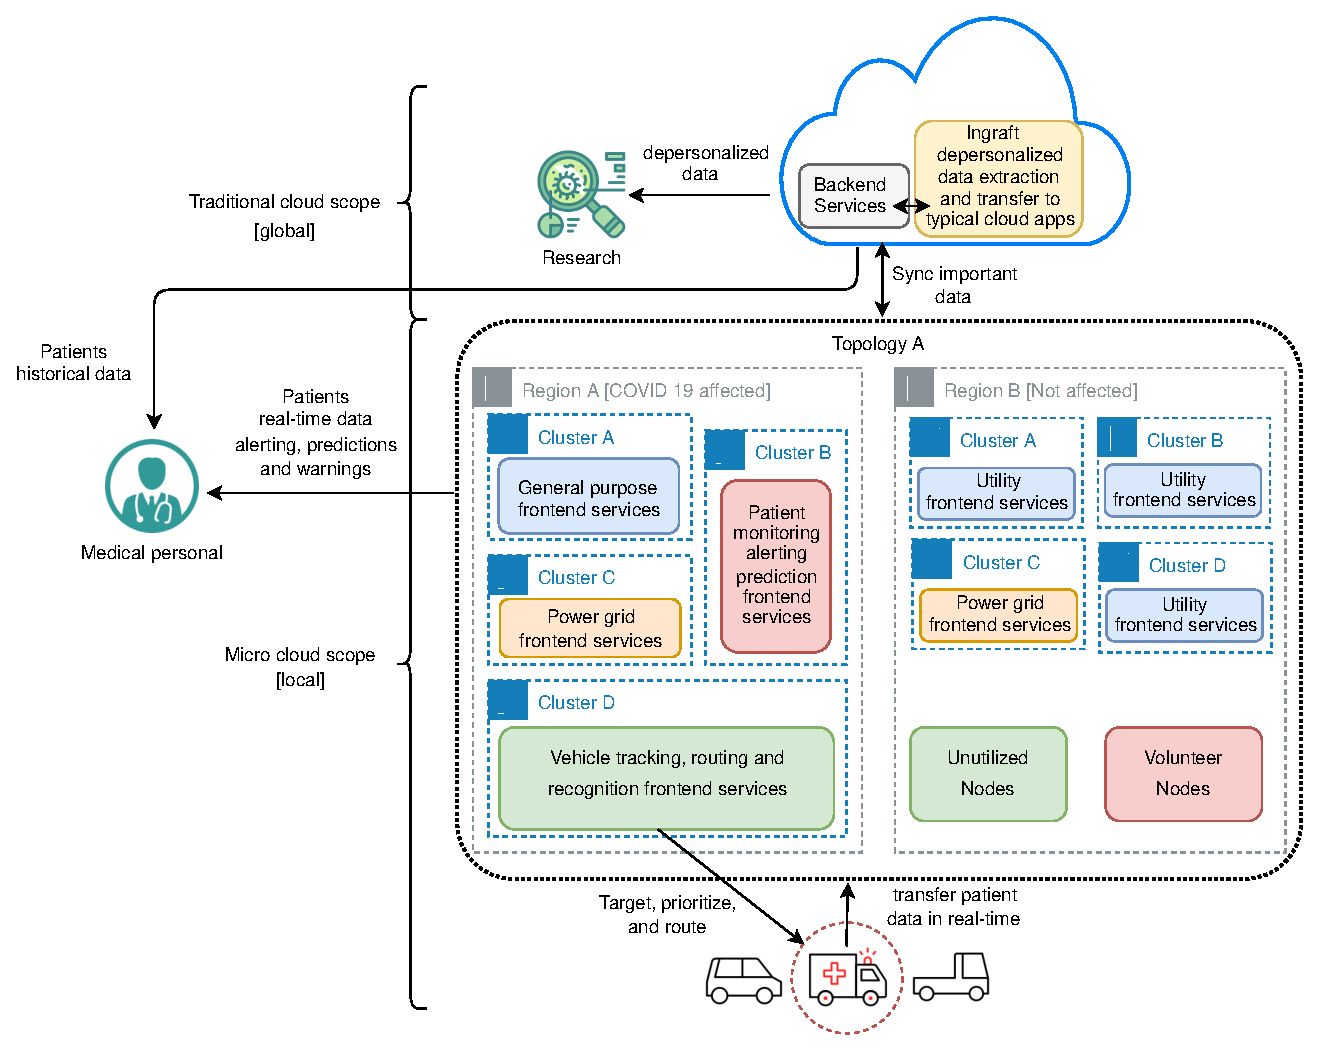
\includegraphics[width=\columnwidth]{images/Figure25}
	\end{center}
	\vspace{-0.5cm}
	\caption{Conceptual architecture model for COVID-19 area traffic control example}
	\label{fig:fig25}
\end{figure}
%
%